\documentclass[number]{ximera}

%My github password is ximera1
%My GeoGebra password is Ximera1

%\usepackage{tikz}

\renewcommand{\theenumi}{\arabic{enumi}.}


% set font encoding for PDFLaTeX, XeLaTeX, or LuaTeX
\usepackage{ifxetex,ifluatex}
\newif\ifxetexorluatex
\ifxetex
  \xetexorluatextrue
\else
  \ifluatex
    \xetexorluatextrue
  \else
    \xetexorluatexfalse
  \fi
\fi

\ifxetexorluatex
  \usepackage{fontspec}
\else
  \usepackage[T1]{fontenc}
  \usepackage[utf8]{inputenc}
  \usepackage{lmodern}
\fi

\usepackage{hyperref}
\usepackage{tikz} %% Adding this here so it's not manually added elsewhere
\title{Angle Sum Formulas - Part I}
\author{Univ. of Minnesota MathCEP}


% Enable SageTeX to run SageMath code right inside this LaTeX file.
% http://mirrors.ctan.org/macros/latex/contrib/sagetex/sagetexpackage.pdf
% \usepackage{sagetex}

\begin{document}

\begin{abstract}
There are many angles that are not one of the standard angles on the unit circle that can, however, be written as a combination of standard angles from the unit circle. For example, $15^\circ = 45^\circ - 30^\circ$, and $75^\circ = 45^\circ + 30^\circ$. The suggests that it would be useful to derive a formula for the sine and cosine of angles that are not one of the standard angles on the unit circle. In this activity, you will apply the distance formula to some wisely-chosen pairs of points to derive formulas for $\cos(A-B)$ and $\cos(A+B)$, where $A$ and $B$ are two arbitrary angles.
\end{abstract}

\maketitle

%7\begin{enumerate} 

For Problems 1-6, find the distance between the given pair of points, paying close attention to the process you are using. Your answers should not contain any decimals.

\begin{problem}
Find the distance between $(4,0)$ and $(-2,0)$.

$\answer{6}$
\end{problem}

\begin{problem}
Find the distance between $(4,3)$ and $(-2,3)$.

$\answer{6}$
\end{problem}

\begin{problem}
Find the distance between $(4,3)$ and $(4,6)$.

$\answer{3}$
\end{problem}

\begin{problem}
Find the distance between $(-2,3)$ and $(4,6)$.

$\answer{\sqrt{45}}$

\begin{hint}
Express your answer without using decimals. What expression would you have typed into a calculator to get your answer? Enter that as your solution instead.
\end{hint}

\end{problem}

\begin{problem}
Find the distance between $(-2,3)$ and $(h,k)$.

$\answer{\sqrt{(-2-h)^2+(3-k)^2}}$

\begin{hint}
Your answer will include the values $h$ and $k$; it cannot be reduced to a number.
\end{hint}

\end{problem}

\begin{problem}
Find the distance between $(x,y)$ and $(h,k)$.

$\answer{\sqrt{(x-h)^2+(y-k)^2}}$

\begin{hint}
Your answer will include the values $x,y,h,$ and $k$.
\end{hint}

\end{problem}

In Problem 6, you deduced a formula for calculating the distance between any two points. We will now apply this formula to certain pairs of points in the plane.

Let $A$ and $B$ be first-quadrant angles with $A>B>(A-B)>0$.

\begin{image}
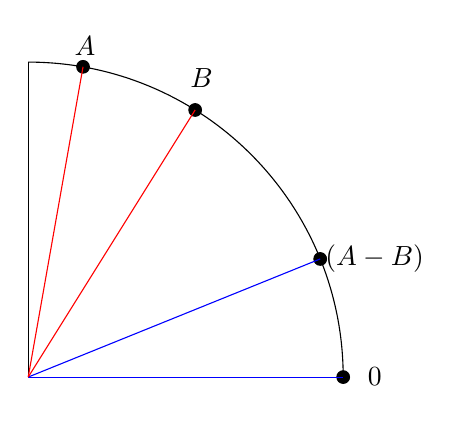
\begin{tikzpicture}[scale=4]

\draw (0,1) arc [radius=1, start angle=90, end angle=0];
\draw [fill] (1,0) circle [radius=0.02];
\draw [fill] (.927,.375) circle [radius=0.02];
\draw [fill] (.174,.985) circle [radius=0.02];
\draw [fill] (.530,.848) circle [radius=0.02];
\draw (0,0) -- (0,1);
\draw [blue] (0,0) -- (1,0);
\draw [blue] (0,0) -- (.927,.375);
\draw [red] (0,0) -- (.174,.985);
\draw [red] (0,0) -- (.530,.848);
\node at (.18,1.05) {$A$};
\node at (.55,.95) {$B$};
\node at (1.1,0.375) {$(A-B)$};
\node at (1.1,0) {$0$};
\end{tikzpicture}
\end{image}

\begin{problem}
Each angle on the unit circle corresponds to a point in the $xy$-plane. For example, the angle of $0$ on the unit circle has the coordinates $(1,0)$. Determine the $(x,y)$-coordinates of where the angles $A,B,$ and $(A-B)$ touch the unit circle.

The $(x,y)$-coordinates associated to angle $A$ are $\left(\answer{\cos(A)},\answer{\sin(A)}\right)$.

The $(x,y)$-coordinates associated to angle $B$ are $\left(\answer{\cos(B)},\answer{\sin(B)}\right)$.

The $(x,y)$-coordinates associated to angle $(A-B)$ are $\left(\answer{\cos(A-B)},\answer{\sin(A-B)}\right)$.
\end{problem}

\begin{problem}
Using the distance formula from Problem 6, set up an expression for the distance between the points associated to angles $A$ and $B$:
\[\sqrt{(\answer{\cos(A)-\cos(B)})^2+(\answer{\sin(A)-\sin(B)})^2}\]
\begin{hint}
There are many variations of the distance formula, all of which are equivalent. One such version is:
\[d((x_1,y_1),(x_2,y_2))=\sqrt{(x_1-x_2)^2+(y_1-y_2)^2}\]
\end{hint}
\end{problem}

\begin{problem}
Using the distance formula from Problem 6, set up an expression for the distance between the points associated to angles $(A-B)$ and $0$:
\[\sqrt{(\answer{\cos(A-B)-1})^2+(\answer{\sin(A-B)-0})^2}\]

\end{problem}

\begin{question}
Explain why the distances found in the previous two Problems are the same.
\begin{freeResponse}

\end{freeResponse}

\end{question}

\begin{problem}
Set the distances in Problems 8 and 9 equal to each other and simplify.
Your result should be a formula for $\cos(A-B)$.

\[\cos(A-B)=\answer{\cos(A)\cos(B)+\sin(A)\sin(B)}\]

\begin{hint}
Your first step should be to square both sides.
\end{hint}
\begin{hint}
Pay close attention to FOILing expressions. Take care to ensure that the angle $(A-B)$ does not get split up.
\end{hint}
\begin{hint}
Look for instances where you can replace expressions of the form $\cos^2(\theta)+\sin^2(\theta)$ with $1$.
\end{hint}
\end{problem}

In Problem 11, you developed an expression for $\cos(A-B)$ in terms of cosine and sine of the angles $A$ and $B$. You will now continue with this to develop an expression for $\cos(A+B)$.

%%%%% I am here!

In order to derive an angle {\bf sum} formula from an angle {\bf difference} formula, you need to be able to write a sum of two values using subtraction.

\begin{problem}
Supply the missing constants:

\begin{itemize}
\item $5-\answer{-3}=8$
\item $2-\answer{-6}=8$
\item $7-\answer{-1}=8$
\end{itemize}
\begin{hint}
If $5-x=8$, adding $x$ and subtracting $8$ from both sides reveals $x=-3$.
\end{hint}

\end{problem}

\begin{problem}
Let $C=-B$. Using your formula from Problem 11, write a formula for $\cos(A-C)$.

\[\cos(A-C)=\answer{\cos(A)\cos(C)+\sin(A)\sin(C)}\]
\end{problem}

\begin{problem}
Which of the following is true about $\cos(C)$?
\begin{selectAll}
\choice[correct]{$\cos(C)=\cos(-B)$}
\choice{$\cos(C)=-\cos(B)$}
\choice[correct]{$\cos(C)=\cos(B)$}
\end{selectAll}

\begin{hint}
Try plugging in values for $C$ and $B$ to test your answers.
\end{hint}

\end{problem}

\begin{problem}
Which of the following is true about $\sin(C)$?
\begin{selectAll}
\choice[correct]{$\sin(C)=\sin(-B)$}
\choice[correct]{$\sin(C)=-\sin(B)$}
\choice{$\sin(C)=\sin(B)$}
\end{selectAll}
\end{problem}

\begin{question}
How does $\cos(C)$ relate to $\cos(B)$? How does $\sin(C)$ relate to $\sin(B)$?
\begin{freeResponse}

\end{freeResponse}
\end{question}

\begin{problem}
In Problem 13, replace $C$ with $-B$:
\[\cos(A--B)= \answer{\cos(A)\cos(-B)+\sin(A)\sin(-B)}\]
\begin{hint}
Take care to not separate the ``$-$'' from $B$.
\end{hint}

\end{problem}

\begin{problem}
Using the relationships explored in Problems 14-16, rewrite the equation from Problem 17 to derive a formula for $\cos(A+B)$:
\[\cos(A+B)=\answer{\cos(A)\cos(B)-\sin(A)\sin(B)}\]
\begin{hint}
It may be useful to factor a negative sign to the front of an expression. For example, $a \times (-b) = -ab$.
\end{hint}

\end{problem}






\end{document}
